%%%%%%%%%%%%%%%%%%%%%%%%
%
% $Autor: Hemanth Jadiswami Prabhakaran $
% $Datum: 2025-06-29 19:44:53Z $
% $Pfad: GitHub/BA25-01-Time-Series/report/Contents/en/seaborn.tex $
% $Version: 1 $
%
% $Project: BA25-Time-Series $
%
%%%%%%%%%%%%%%%%%%%%%%%%


%
% !TeX encoding = utf8
% !TeX root = PythonPackages
%
%%%%%%%%%%%%%%%%%%%%%%%%

\chapter{Seaborn}
\label{ch:seaborn}

\section{Introduction}
\label{sec:intro}

Seaborn is a powerful statistical data visualization library built on top of matplotlib, designed to make statistical plotting in Python both beautiful and informative \cite{Seaborn:2024}. Created by Michael Waskom, Seaborn provides a high-level interface for drawing attractive and informative statistical graphics. The library excels at creating complex visualizations with minimal code while maintaining aesthetic appeal and statistical rigor \cite{Waskom:2021}. This chapter provides comprehensive coverage of Seaborn's capabilities, from basic plotting to advanced statistical visualizations, demonstrating how to create publication-ready graphics for data analysis and scientific communication.\\

The significance of Seaborn in the data visualization ecosystem stems from its focus on statistical graphics and its integration with the broader scientific Python ecosystem. While matplotlib provides fine-grained control over plot elements, Seaborn offers intelligent defaults and statistical functionality that streamlines the creation of complex visualizations \cite{Seaborn:2024}. Modern data science workflows benefit from Seaborn's ability to quickly explore relationships in data through built-in statistical functions, color palettes, and plot types specifically designed for statistical analysis \cite{VanderPlas:2023}. The library's emphasis on both aesthetics and statistical accuracy has made it an essential tool for data scientists, researchers, and analysts worldwide.\\

\section{Description}
\label{sec:description}

\subsection{Core Capabilities}
\label{subsec:capabilities}

Seaborn offers a comprehensive suite of statistical visualization capabilities:

\begin{itemize}
	\item \textbf{Statistical Plotting}: Built-in statistical functions for regression, distribution, and categorical data analysis
	\item \textbf{Beautiful Defaults}: Aesthetically pleasing default styles and color palettes
	\item \textbf{DataFrame Integration}: Native pandas DataFrame support for seamless data handling
	\item \textbf{Multi-plot Grids}: Faceted plotting for exploring relationships across data subsets
	\item \textbf{Customization}: Extensive theming and customization options built on matplotlib
\end{itemize}

\clearpage

\subsection{Python Framework: seaborn}
\label{subsec:seaborn}

The \texttt{seaborn} package provides an intuitive interface for statistical visualization:

\begin{lstlisting}[language=MyPython, caption={Seaborn Core Functions}, label={lst:seaborn_core}]
	
	import seaborn as sns
	import matplotlib.pyplot as plt
	import pandas as pd
	
	# Load sample data
	tips = sns.load_dataset("tips")
	
	# Create statistical visualizations
	sns.scatterplot(data=tips, x="total_bill", y="tip", hue="time")
	sns.regplot(data=tips, x="total_bill", y="tip")
	sns.boxplot(data=tips, x="day", y="total_bill")
	
	plt.show()
	
\end{lstlisting}

\subsection{Use Cases}
\label{subsec:usecases}

Seaborn finds applications across diverse analytical domains:

\begin{enumerate}
	\item \textbf{Exploratory Data Analysis}: Quick visualization of data distributions and relationships
	\item \textbf{Statistical Analysis}: Regression plots, correlation matrices, and distribution analysis
	\item \textbf{Research Publications}: Publication-quality statistical graphics
	\item \textbf{Business Intelligence}: Dashboard creation and data storytelling
	\item \textbf{Machine Learning}: Feature analysis and model interpretation visualization
\end{enumerate}

\subsection{Architecture Overview}
\label{subsec:architecture}

\begin{figure}[H]
	\centering
	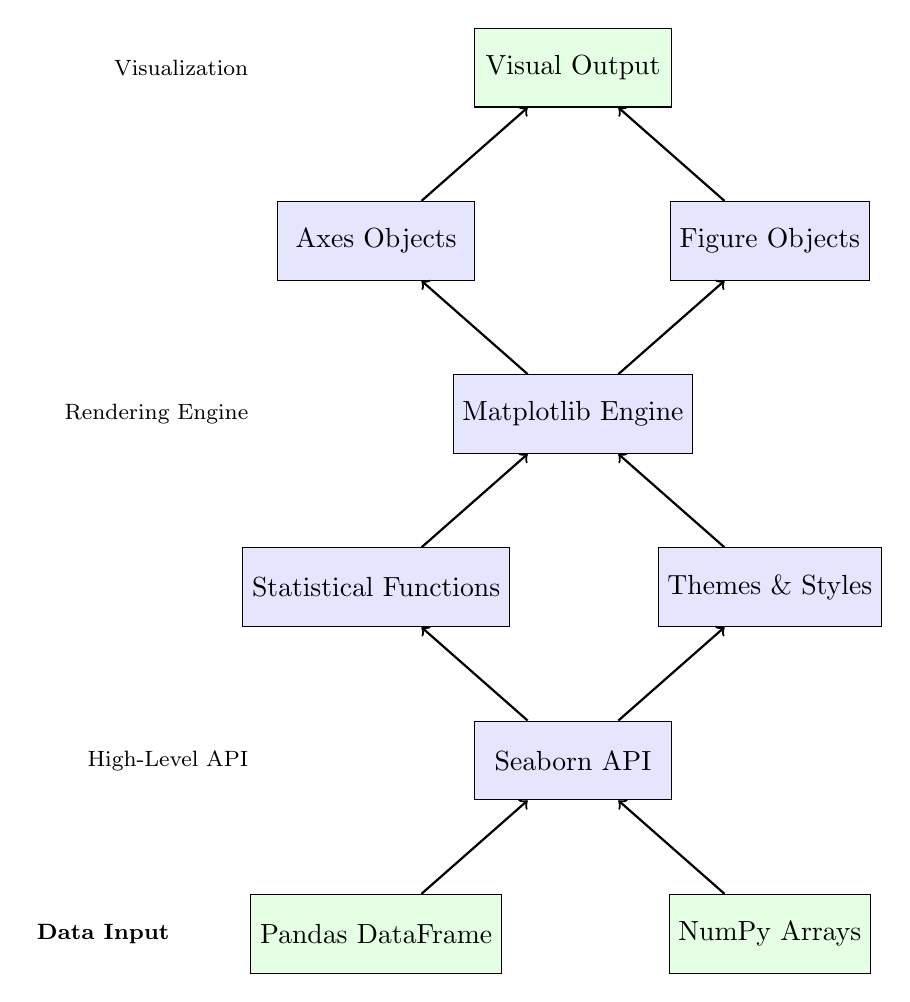
\begin{tikzpicture}[
	box/.style={rectangle, draw, fill=blue!10, minimum width=2.5cm, minimum height=1cm, text centered},
	data/.style={rectangle, draw, fill=green!10, minimum width=2.5cm, minimum height=1cm, text centered},
	arrow/.style={thick, ->}
	]
	
	% Data Layer (moved further apart)
	\node[data] (data) at (-2.5,0) {Pandas DataFrame};
	\node[data] (numpy) at (2.5,0) {NumPy Arrays};
	
	% Seaborn Layer
	\node[box] (seaborn) at (0,2.2) {Seaborn API};
	\node[box] (stats) at (-2.5,4.4) {Statistical Functions};
	\node[box] (themes) at (2.5,4.4) {Themes \& Styles};
	
	% Matplotlib Layer
	\node[box] (matplotlib) at (0,6.6) {Matplotlib Engine};
	\node[box] (axes) at (-2.5,8.8) {Axes Objects};
	\node[box] (figures) at (2.5,8.8) {Figure Objects};
	
	% Output Layer
	\node[data] (output) at (0,11) {Visual Output};
	
	% Arrows
	\draw[arrow] (data) -- (seaborn);
	\draw[arrow] (numpy) -- (seaborn);
	\draw[arrow] (seaborn) -- (stats);
	\draw[arrow] (seaborn) -- (themes);
	\draw[arrow] (stats) -- (matplotlib);
	\draw[arrow] (themes) -- (matplotlib);
	\draw[arrow] (matplotlib) -- (axes);
	\draw[arrow] (matplotlib) -- (figures);
	\draw[arrow] (axes) -- (output);
	\draw[arrow] (figures) -- (output);
	
	% Layer Labels (aligned to left of the leftmost node)
	\node[left] at (-5,0) {\footnotesize \textbf{Data Input}};
	\node[left] at (-4,2.2) {\footnotesize High-Level API};
	\node[left] at (-4,6.6) {\footnotesize Rendering Engine};
	\node[left] at (-4,11) {\footnotesize Visualization};
	
\end{tikzpicture}
	\caption{Seaborn Visualization Architecture \cite{Seaborn:2024}}
	\label{fig:seaborn_architecture}
\end{figure}

The Seaborn architecture builds upon matplotlib's foundation, as illustrated in Figure \ref{fig:seaborn_architecture}. Seaborn acts as a high-level interface that processes pandas DataFrames through statistical functions and renders them using matplotlib's plotting engine. This layered approach provides both statistical sophistication and visual appeal \cite{Waskom:2021}.

\clearpage

\section{Installation}
\label{sec:installation}

\subsection{System Requirements}
\label{subsec:system_requirements}

Seaborn requires Python 3.7 or higher and depends on several scientific computing libraries including NumPy, pandas, and matplotlib. The library works across all major operating systems with minimal system-specific requirements.

\subsection{Python Package Installation}
\label{subsec:python_install}

Install Seaborn using pip or conda:

\begin{lstlisting}[style=bashstyle, caption={Seaborn Installation}]
	# Basic installation via pip
	pip install seaborn
	
	# Installation with all dependencies
	pip install seaborn pandas matplotlib numpy scipy
	
	# Installation via conda (recommended for scientific computing)
	conda install seaborn
	
	# Development version from GitHub
	pip install git+https://github.com/mwaskom/seaborn.git
\end{lstlisting}

\subsection{Verification}
\label{subsec:verification}

Verify the installation by creating a simple plot:

\begin{lstlisting}[language=MyPython, caption={Seaborn Installation Verification}]
	import seaborn as sns
	import matplotlib.pyplot as plt
	
	# Create a simple plot with sample data
	tips = sns.load_dataset("tips")
	sns.scatterplot(data=tips, x="total_bill", y="tip")
	plt.show()
	
	print(f"Seaborn version: {sns.__version__}")
\end{lstlisting}

\section{Example -- Statistical Data Exploration}
\label{sec:basic_example}

The following example demonstrates basic statistical visualization capabilities. The complete implementation is available in \texttt{BasicVisualization.py}.

\lstinputlisting[language=MyPython, caption={Basic Statistical Visualization}, label={lst:basicviz},firstline=1,lastline=50]{../Code/seaborn/BasicVisualization.py}

\noindent\textit{[The remaining code is omitted for brevity. The complete script can be found at \texttt{../Code/seaborn/BasicVisualization.py}.]}

This example showcases Seaborn's ability to create multiple types of statistical plots with minimal code, demonstrating the library's strength in exploratory data analysis.

\section{Example -- Advanced Statistical Analysis}
\label{sec:advanced_example}

Advanced Seaborn applications leverage multi-plot grids and custom styling for comprehensive data analysis. The integration of statistical functions enables sophisticated analytical visualizations.

\clearpage

\begin{figure}[htbp]
	\centering
    \begin{tikzpicture}[
	process/.style={rectangle, draw, fill=blue!10, minimum width=2cm, minimum height=0.8cm, text centered},
	data/.style={ellipse, draw, fill=green!10, minimum width=1.8cm, minimum height=0.8cm, text centered},
	arrow/.style={thick, ->}
	]
	
	% Vertical flow from top to bottom
	\node[data] (input) at (0,3) {Raw Data};
	\node[process] (load) at (0,2) {Load \& Clean};
	\node[process] (analyze) at (0,1) {Statistical Analysis};
	\node[data] (output) at (0,0) {Visualization};
	
	% Flow arrows
	\draw[arrow] (input) -- (load);
	\draw[arrow] (load) -- (analyze);
	\draw[arrow] (analyze) -- (output);
	
	% Tool labels
\node[right] at (2,2) {\footnotesize pandas};
\node[right] at (2,1) {\footnotesize seaborn};
\node[right] at (2,0) {\footnotesize matplotlib};
	
	% Process details
	\node[left] at (-2,2) {\footnotesize Data prep};
	\node[left] at (-2,1) {\footnotesize Plot creation};
	
\end{tikzpicture}
	\caption{Statistical Analysis Workflow with Seaborn}
	\label{fig:statistical_workflow}
\end{figure}

The statistical workflow illustrated in Figure \ref{fig:statistical_workflow} shows the progression from data input through exploratory analysis to final visualization output.

\lstinputlisting[language=MyPython, caption={Advanced Statistical Analysis}, label={lst:advancedstats},firstline=1,lastline=50]{../Code/seaborn/AdvancedAnalysis.py}
\noindent\textit{The remaining code is omitted for brevity. The complete script can be found at \texttt{../Code/seaborn/AdvancedAnalysis.py}.}

\section{Example -- Publication-Quality Visualizations}
\label{sec:publication_example}

Seaborn excels at creating publication-ready visualizations with professional styling and statistical rigor. The framework's theming system enables consistent, high-quality graphics suitable for academic and professional publication.

\begin{figure}[htbp]
	\centering
    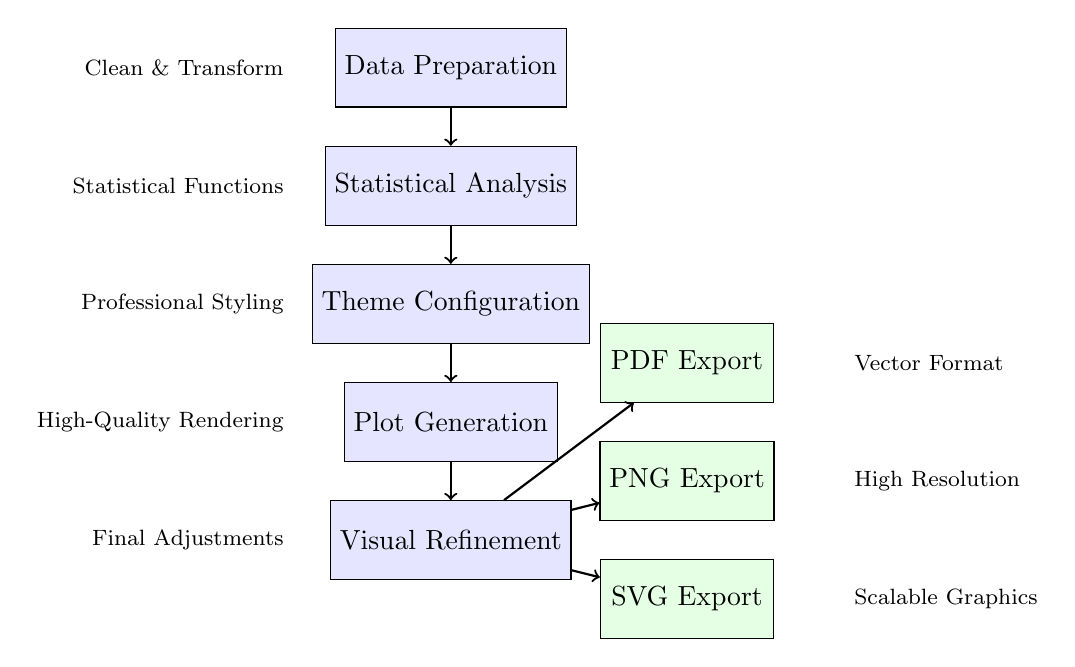
\begin{tikzpicture}[
    stage/.style={rectangle, draw, fill=blue!10, minimum width=2.2cm, minimum height=1cm, text centered},
    output/.style={rectangle, draw, fill=green!10, minimum width=2.2cm, minimum height=1cm, text centered},
    arrow/.style={thick, ->}
]

% Vertical pipeline layout
\node[stage] (data) at (0,6) {Data Preparation};
\node[stage] (analysis) at (0,4.5) {Statistical Analysis};
\node[stage] (styling) at (0,3) {Theme Configuration};
\node[stage] (plotting) at (0,1.5) {Plot Generation};
\node[stage] (refinement) at (0,0) {Visual Refinement};

% Output formats
\node[output] (pdf) at (3,2.25) {PDF Export};
\node[output] (png) at (3,0.75) {PNG Export};
\node[output] (svg) at (3,-0.75) {SVG Export};

% Process flow
\draw[arrow] (data) -- (analysis);
\draw[arrow] (analysis) -- (styling);
\draw[arrow] (styling) -- (plotting);
\draw[arrow] (plotting) -- (refinement);

% Output arrows
\draw[arrow] (refinement) -- (pdf);
\draw[arrow] (refinement) -- (png);
\draw[arrow] (refinement) -- (svg);

% Side annotations
\node[left] at (-2,6) {\footnotesize Clean \& Transform};
\node[left] at (-2,4.5) {\footnotesize Statistical Functions};
\node[left] at (-2,3) {\footnotesize Professional Styling};
\node[left] at (-2,1.5) {\footnotesize High-Quality Rendering};
\node[left] at (-2,0) {\footnotesize Final Adjustments};

% Quality indicators
\node[right] at (5,2.25) {\footnotesize Vector Format};
\node[right] at (5,0.75) {\footnotesize High Resolution};
\node[right] at (5,-0.75) {\footnotesize Scalable Graphics};

\end{tikzpicture}
	\caption{Publication Visualization Pipeline}
	\label{fig:publication_pipeline}
\end{figure}

The publication pipeline illustrated in Figure \ref{fig:publication_pipeline} demonstrates the workflow from raw data to publication-ready statistical graphics.

\lstinputlisting[language=MyPython, caption={Publication-Quality Visualizations}, label={lst:publication},firstline=1,lastline=50]{../Code/seaborn/PublicationPlots.py}

\noindent\textit{[The remaining code is omitted for brevity. The complete script can be found at \texttt{../Code/seaborn/PublicationPlots.py}.]}

\section{Example -- Custom Styling and Themes}
\label{sec:styling_example}

Seaborn provides extensive customization options for creating branded or themed visualizations. The styling system enables consistent visual identity across multiple plots and publications.

\lstinputlisting[language=MyPython, caption={Custom Styling and Themes}, label={lst:styling},firstline=1,lastline=50]{../Code/seaborn/CustomStyling.py}

\noindent\textit{[The remaining code is omitted for brevity. The complete script can be found at \texttt{../Code/seaborn/CustomStyling.py}.]}

\section{Performance Optimization}
\label{sec:optimization}

Optimizing Seaborn visualizations requires understanding data preprocessing, plot complexity management, and efficient rendering techniques. Proper optimization ensures responsive visualization creation even with large datasets.

\subsection{Data Preprocessing Strategies}
\label{subsec:preprocessing}

Efficient data handling for improved visualization performance:

\begin{lstlisting}[language=MyPython, caption={Data Preprocessing for Performance}, label={lst:preprocessing}]
	import pandas as pd
	import seaborn as sns
	
	# Optimize data types before plotting
	def optimize_dataframe(df):
	    for col in df.select_dtypes(include=['int64']).columns:
	        df[col] = pd.to_numeric(df[col], downcast='integer')
	    for col in df.select_dtypes(include=['float64']).columns:
	        df[col] = pd.to_numeric(df[col], downcast='float')
	    return df
	
	# Sample large datasets for quick exploration
	def sample_for_plotting(df, max_points=10000):
	    if len(df) > max_points:
	        return df.sample(n=max_points, random_state=42)
	    return df
\end{lstlisting}

\subsection{Rendering Optimization}
\label{subsec:rendering}

Techniques for efficient plot rendering and display:

\begin{lstlisting}[language=MyPython, caption={Rendering Optimization}, label={lst:rendering}]
	import matplotlib.pyplot as plt
	import seaborn as sns
	
	# Configure matplotlib backend for performance
	plt.ioff()  # Turn off interactive mode
	
	# Use appropriate figure sizes
	sns.set_context("paper", font_scale=1.2)
	
	# Optimize for specific output formats
	def save_optimized_plot(filename, dpi=300):
	    plt.savefig(filename, dpi=dpi, bbox_inches='tight',
	                facecolor='white', edgecolor='none')
	    plt.close()  # Free memory
\end{lstlisting}

\section{Error Handling and Best Practices}
\label{sec:best_practices}

Robust Seaborn applications must handle data quality issues, missing values, and visualization complexity. Implementing proper error handling ensures reliable visualization generation across diverse datasets.

\subsection{Common Issues and Solutions}
\label{subsec:common_issues}

\begin{enumerate}
	\item \textbf{Missing Data}: Handle NaN values appropriately for different plot types
	\item \textbf{Large Datasets}: Implement sampling strategies for interactive exploration
	\item \textbf{Memory Usage}: Manage figure objects and clear plots after saving
	\item \textbf{Color Mapping}: Ensure sufficient color contrast and accessibility
\end{enumerate}

\subsection{Error Handling Patterns}
\label{subsec:error_patterns}

\lstinputlisting[language=MyPython, caption={Comprehensive Error Handling with Seaborn}, label={lst:seaborn_errorhandling},firstline=1,lastline=50]{../Code/seaborn/ErrorHandling.py}

\noindent\textit{[The remaining code is omitted for brevity. The complete script can be found at \texttt{../Code/seaborn/ErrorHandling.py}.]}

\section{Further Reading}
\label{sec:further_reading}

To deepen understanding of Seaborn and statistical visualization, consider these resources:

\subsection{Official Documentation}
\begin{itemize}
	\item \textbf{Seaborn Documentation}: \url{https://seaborn.pydata.org/}
	\item \textbf{Seaborn Tutorial}: \url{https://seaborn.pydata.org/tutorial.html}
	\item \textbf{Seaborn GitHub Repository}: Official source code repository \cite{Seaborn:2024}
	\item \textbf{Seaborn Gallery}: \url{https://seaborn.pydata.org/examples/index.html}
	\item \textbf{Statistical Visualization Guide}: \url{https://seaborn.pydata.org/tutorial/introduction.html}
\end{itemize}

\subsection{Tutorials and Guides}
\begin{itemize}
	\item \href{https://jakevdp.github.io/PythonDataScienceHandbook/}{Python Data Science Handbook} \cite{VanderPlas:2023}
	\item \href{https://www.python-graph-gallery.com/seaborn/}{Python Graph Gallery - Seaborn Section}
	\item \href{https://towardsdatascience.com/data-visualisation-tutorial-using-seaborn-26e1ef9043db/}{Comprehensive Seaborn Tutorial} \cite{TowardsSeaborn:2023}
\end{itemize}

\section{Conclusion}
\label{sec:conclusion}

Seaborn provides an essential toolkit for statistical data visualization in Python, combining aesthetic appeal with statistical rigor. From exploratory data analysis to publication-quality graphics, Seaborn's intuitive API and comprehensive feature set make it indispensable for data scientists and researchers. The examples and techniques presented in this chapter demonstrate the library's versatility and power, while the architectural understanding enables effective integration into diverse analytical workflows.\\

Future developments in Seaborn focus on enhanced statistical functions, improved performance with large datasets, and expanded customization options \cite{Waskom:2021}. As the field of data visualization continues to evolve, Seaborn remains at the forefront of statistical graphics, providing researchers and analysts worldwide with the tools needed to create compelling and informative visualizations that drive insight and understanding.